\documentclass[titlepage, 12pt, twoside, openright, a4paper]{report}

% ----------------------- PACKAGES -----------------------

% Setting margins
\usepackage[margin=20mm]{geometry}
% Sets paragraphs to skip a line rather than indent
\usepackage{parskip}
% H float modifier
\usepackage{float}
% For graphs and plots
\usepackage{pgfplots}
% For code listings
\usepackage{listings}
% Fort for code listings
\usepackage{inconsolata}
% Additional mathematical typesetting features
\usepackage{amsmath, amsfonts}
% Prevents page numbers from appearing on empty pages (still counts the page)
\usepackage{emptypage}
% Linked table of contents.
\usepackage{bookmark}
% Colours
\usepackage{xcolor}

% ----------------------- SETTINGS -----------------------

% Code listings configuration
\definecolor{codebackgroundcolour}{rgb}{0.9, 0.9, 0.9}

\lstset{
    basicstyle=\ttfamily,
    columns=fullflexible,
    breaklines=true,
    backgroundcolor=\color{codebackgroundcolour},
    framesep=5pt,
    frame=tlbr,
    framerule=0pt
}


% Sans serif computer modern font as default for text
\renewcommand{\familydefault}{\sfdefault}

% Force version of pdfplots
\pgfplotsset{compat=1.18}

% Allows filling colours between curves
\usepgfplotslibrary{fillbetween}


% ----------------------- MACROS -----------------------

% For large comments
\newcommand{\comment}[1]{}

% Creates a new chapter with vertical space correctly
\newcommand{\newchapter}[1]{\chapter{#1}\vspace{17\baselineskip}}

% Takes as arguments: label, width, path
\newcommand{\centeredimage}[3]{\begin{figure}[H]\centering\label{#1}\includegraphics[width=#2]{#3}\end{figure}}

% ----------------------- DOCUMENT -----------------------

\title{Latex Book Template}
\author{Aaron Manning}
\date{}

\begin{document}

    \maketitle
    \tableofcontents

    % Allows display maths to be broken up across pages
    \allowdisplaybreaks

    % Ragged right text, resolves many hbox overfull issues
    \raggedright

    % ----------------------- CHAPTERS -----------------------

    \newchapter{Examples}

\section{Section}
This is a section, which is the second highest level behind a chapter.

\subsection{Subsection}
This is a subsection, which is one level below it. Notice the numbering of the subsection compared to the chapter and section.

\subsubsection{Subsubsection}
This is a subsubsection, which doesn't appear in the table of contents and doesn't have a number, but gives a sensible way to separate text with a bold header.

\section{Paragraph Text}

Lorem ipsum dolor sit amet, consectetur adipiscing elit. Aenean ac quam eu eros placerat volutpat. Nulla facilisi. Nulla nunc orci, pellentesque et nisi sed, ornare viverra massa. Sed vel nunc urna. Nullam vehicula sed augue eget finibus. Donec vitae varius ipsum. In hac habitasse platea dictumst. Fusce efficitur nunc vitae urna venenatis, et mattis turpis facilisis. Vivamus sagittis neque enim, vitae tempor nisi imperdiet a. Mauris sit amet auctor lectus, quis feugiat ipsum. Donec in scelerisque erat, sed efficitur sapien. Nam fringilla ante massa, in elementum dui consequat bibendum. Suspendisse dapibus at lectus euismod laoreet. Pellentesque rutrum nisi a libero pulvinar sollicitudin. Mauris hendrerit lacus at feugiat auctor. Pellentesque a quam eget eros condimentum ultrices et eu enim.

Cras lacinia tempus arcu, eu sollicitudin lacus placerat sed. Nunc eleifend laoreet placerat. Nulla lectus augue, consequat in laoreet vitae, euismod eu eros. Nullam fringilla nunc sem, sed ornare ipsum tempor nec. Morbi hendrerit augue eget purus egestas, sit amet iaculis velit scelerisque. Praesent nunc purus, convallis non pellentesque quis, scelerisque hendrerit libero. Fusce quis auctor ligula, vel viverra nulla. In in nisl sit amet libero pharetra semper ac nec ex. Donec porttitor sem a tellus euismod, at fringilla neque sagittis. Praesent varius magna vitae velit ornare, vel blandit metus malesuada. Suspendisse blandit orci nec arcu pharetra pretium. Pellentesque malesuada, mi quis finibus malesuada, nunc nibh viverra quam, blandit malesuada neque nulla vel ipsum. Curabitur vestibulum in risus ut laoreet. Nam placerat id ante ut efficitur. Ut euismod tellus id ante egestas, vitae viverra arcu gravida.

Nunc et iaculis risus, id rhoncus quam. Vestibulum sed quam sed dui scelerisque rutrum sed nec lectus. Pellentesque condimentum, massa et aliquet eleifend, libero elit vulputate lacus, id convallis neque est a tortor. Phasellus id sapien luctus, ultrices mi sit amet, condimentum neque. Suspendisse nisi sem, elementum vel nulla ac, mattis faucibus diam. Aenean blandit tellus eget odio malesuada consectetur. Class aptent taciti sociosqu ad litora torquent per conubia nostra, per inceptos himenaeos. Nunc dictum tincidunt pharetra. Pellentesque habitant morbi tristique senectus et netus et malesuada fames ac turpis egestas. Ut convallis mi urna, ut aliquet justo rhoncus laoreet. Nam vestibulum tortor et velit ullamcorper placerat. Integer id felis a sem pellentesque viverra. Etiam eros leo, ornare vel risus sit amet, accumsan sagittis velit. Sed commodo libero nulla, sit amet porta lectus congue at. Integer ac est suscipit, pharetra dui nec, eleifend elit. Fusce enim neque, efficitur ut quam id, volutpat congue justo.

Aliquam aliquet finibus nisi, dictum malesuada dui ultrices non. Vestibulum a elit blandit, ornare dolor vel, aliquam sem. Pellentesque eu risus sapien. Curabitur dolor est, egestas at turpis ac, imperdiet pretium lectus. Nunc sollicitudin lobortis orci. Proin dapibus ornare tellus, viverra convallis urna dignissim aliquet. Orci varius natoque penatibus et magnis dis parturient montes, nascetur ridiculus mus.

In vitae nisi egestas, auctor enim vitae, fermentum velit. Proin lectus mauris, posuere in sodales a, tempus vitae velit. Fusce congue maximus dolor, sed varius enim viverra vel. Aliquam sodales laoreet mauris id tempor. In convallis est a malesuada semper. Proin porta dui ligula, eu auctor augue ornare dapibus. In volutpat hendrerit tellus eu pellentesque. Aliquam aliquam nisl quis luctus sollicitudin. Nam sagittis nisi dapibus, aliquam risus id, maximus est. Suspendisse diam arcu, tincidunt eu tincidunt id, venenatis non mi. Vestibulum ut sapien vitae diam luctus vestibulum ut sed felis.

\newpage

\section{Code Listings}

Here is what a code listing looks like by default.

\begin{lstlisting}
#include <stdio.h>

int main() {
    printf("Hello, World!\n");
    return 0;
}
\end{lstlisting}



\section{Mathematics}

Here are some sample mathematical expressions and equations, typeset properly.

\[
    \overline{x} = \frac{1}{n} \sum_{i = 1}^{n} x_{i}
\]

\begin{align*}
    \frac{d}{d\theta} \left( \cos(\theta) + i\sin(\theta) \right) &= -\sin(\theta) + i\cos(\theta) \\
    &= i(\cos(\theta) + i\sin(\theta))
\end{align*}


\section{Images}

There is a command for including central images at the current location easily.

\centeredimage{Sample}{10cm}{images/sample.png}

\section{Plots}

Plots are very easy to make using pgfplots:

\begin{center}
    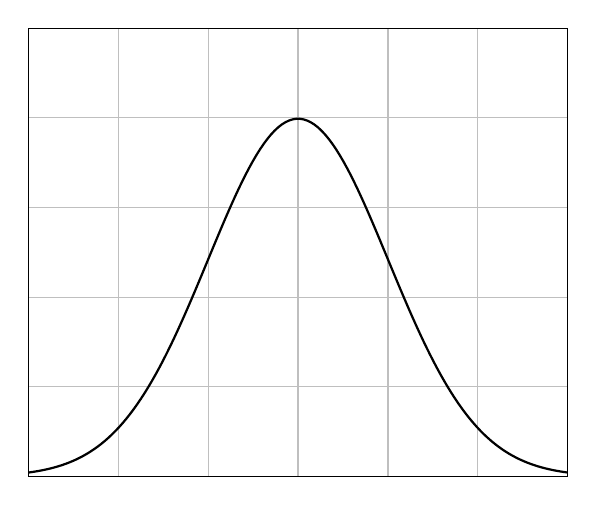
\begin{tikzpicture}
        \begin{axis}[xmin=-3,ymin=0,xmax=3,ymax=0.5,samples=250,grid=major,ticks=none,xlabel={},ylabel={},title={}]
            \addplot[black, thick]{(1/(2 * 3.1415)^(1/2)) * e^(-(x^2)/2 };
        \end{axis}
    \end{tikzpicture}
\end{center}

\section{Tables}

Here is an example of a table as well:

\begin{table}[ht]
    \centering
    \begin{tabular}{rrrrrrrrrrr}
      \hline
    \(z\) & 0 & .01 & .02 & .03 & .04 & .05 & .06 & .07 & .08 & .09 \\
      \hline
    -3.0 & 0.0013 & 0.0013 & 0.0013 & 0.0012 & 0.0012 & 0.0011 & 0.0011 & 0.0011 & 0.0010 & 0.0010 \\ 
      -2.9 & 0.0019 & 0.0018 & 0.0018 & 0.0017 & 0.0016 & 0.0016 & 0.0015 & 0.0015 & 0.0014 & 0.0014 \\
      -2.8 & 0.0026 & 0.0025 & 0.0024 & 0.0023 & 0.0023 & 0.0022 & 0.0021 & 0.0021 & 0.0020 & 0.0019 \\
      -2.7 & 0.0035 & 0.0034 & 0.0033 & 0.0032 & 0.0031 & 0.0030 & 0.0029 & 0.0028 & 0.0027 & 0.0026 \\
      -2.6 & 0.0047 & 0.0045 & 0.0044 & 0.0043 & 0.0041 & 0.0040 & 0.0039 & 0.0038 & 0.0037 & 0.0036 \\
      -2.5 & 0.0062 & 0.0060 & 0.0059 & 0.0057 & 0.0055 & 0.0054 & 0.0052 & 0.0051 & 0.0049 & 0.0048 \\
      -2.4 & 0.0082 & 0.0080 & 0.0078 & 0.0075 & 0.0073 & 0.0071 & 0.0069 & 0.0068 & 0.0066 & 0.0064 \\
      -2.3 & 0.0107 & 0.0104 & 0.0102 & 0.0099 & 0.0096 & 0.0094 & 0.0091 & 0.0089 & 0.0087 & 0.0084 \\
      -2.2 & 0.0139 & 0.0136 & 0.0132 & 0.0129 & 0.0125 & 0.0122 & 0.0119 & 0.0116 & 0.0113 & 0.0110 \\
      -2.1 & 0.0179 & 0.0174 & 0.0170 & 0.0166 & 0.0162 & 0.0158 & 0.0154 & 0.0150 & 0.0146 & 0.0143 \\
      -2.0 & 0.0228 & 0.0222 & 0.0217 & 0.0212 & 0.0207 & 0.0202 & 0.0197 & 0.0192 & 0.0188 & 0.0183 \\
      -1.9 & 0.0287 & 0.0281 & 0.0274 & 0.0268 & 0.0262 & 0.0256 & 0.0250 & 0.0244 & 0.0239 & 0.0233 \\
      -1.8 & 0.0359 & 0.0351 & 0.0344 & 0.0336 & 0.0329 & 0.0322 & 0.0314 & 0.0307 & 0.0301 & 0.0294 \\
      -1.7 & 0.0446 & 0.0436 & 0.0427 & 0.0418 & 0.0409 & 0.0401 & 0.0392 & 0.0384 & 0.0375 & 0.0367 \\
      -1.6 & 0.0548 & 0.0537 & 0.0526 & 0.0516 & 0.0505 & 0.0495 & 0.0485 & 0.0475 & 0.0465 & 0.0455 \\
      -1.5 & 0.0668 & 0.0655 & 0.0643 & 0.0630 & 0.0618 & 0.0606 & 0.0594 & 0.0582 & 0.0571 & 0.0559 \\
      -1.4 & 0.0808 & 0.0793 & 0.0778 & 0.0764 & 0.0749 & 0.0735 & 0.0721 & 0.0708 & 0.0694 & 0.0681 \\
      -1.3 & 0.0968 & 0.0951 & 0.0934 & 0.0918 & 0.0901 & 0.0885 & 0.0869 & 0.0853 & 0.0838 & 0.0823 \\
      -1.2 & 0.1151 & 0.1131 & 0.1112 & 0.1093 & 0.1075 & 0.1056 & 0.1038 & 0.1020 & 0.1003 & 0.0985 \\
      -1.1 & 0.1357 & 0.1335 & 0.1314 & 0.1292 & 0.1271 & 0.1251 & 0.1230 & 0.1210 & 0.1190 & 0.1170 \\
      -1.0 & 0.1587 & 0.1562 & 0.1539 & 0.1515 & 0.1492 & 0.1469 & 0.1446 & 0.1423 & 0.1401 & 0.1379 \\
      -0.9 & 0.1841 & 0.1814 & 0.1788 & 0.1762 & 0.1736 & 0.1711 & 0.1685 & 0.1660 & 0.1635 & 0.1611 \\
      -0.8 & 0.2119 & 0.2090 & 0.2061 & 0.2033 & 0.2005 & 0.1977 & 0.1949 & 0.1922 & 0.1894 & 0.1867 \\
      -0.7 & 0.2420 & 0.2389 & 0.2358 & 0.2327 & 0.2296 & 0.2266 & 0.2236 & 0.2206 & 0.2177 & 0.2148 \\
      -0.6 & 0.2743 & 0.2709 & 0.2676 & 0.2643 & 0.2611 & 0.2578 & 0.2546 & 0.2514 & 0.2483 & 0.2451 \\
      -0.5 & 0.3085 & 0.3050 & 0.3015 & 0.2981 & 0.2946 & 0.2912 & 0.2877 & 0.2843 & 0.2810 & 0.2776 \\
      -0.4 & 0.3446 & 0.3409 & 0.3372 & 0.3336 & 0.3300 & 0.3264 & 0.3228 & 0.3192 & 0.3156 & 0.3121 \\
      -0.3 & 0.3821 & 0.3783 & 0.3745 & 0.3707 & 0.3669 & 0.3632 & 0.3594 & 0.3557 & 0.3520 & 0.3483 \\
      -0.2 & 0.4207 & 0.4168 & 0.4129 & 0.4090 & 0.4052 & 0.4013 & 0.3974 & 0.3936 & 0.3897 & 0.3859 \\
      -0.1 & 0.4602 & 0.4562 & 0.4522 & 0.4483 & 0.4443 & 0.4404 & 0.4364 & 0.4325 & 0.4286 & 0.4247 \\
      0 & 0.5000 & 0.4960 & 0.4920 & 0.4880 & 0.4840 & 0.4801 & 0.4761 & 0.4721 & 0.4681 & 0.4641 \\ 
       \hline
    \end{tabular}
\end{table}


\end{document}